\section{Experiment 3: Position-Length}
\label{sec:positionlength}

Cleveland and McGill assess the perception of position and length across five designs of grouped and divided bar charts (Fig.~\ref{fig:figure4_mlae}). Both types of chart can show the same information, but the elementary perceptual task is different: a grouped bar chart always involves the judgment of positions along a common scale, while a divided bar chart also requires length judgments. Types 1, 2, and 3 involve relating the judgment of positions along a common scale while types 4 and 5 involve relating the measure of length. For each graph, two bars or bar segments were marked, and participants were asked to judge what percentage the smaller marked element was of the larger. Cleveland and McGill ordered the types from easiest (type 1) to hardest (type 5).

\setlength{\belowdisplayskip}{3pt} \setlength{\belowdisplayshortskip}{3pt}
\setlength{\abovedisplayskip}{3pt} \setlength{\abovedisplayshortskip}{3pt}

For data generation, we follow the same approach as in the original experiment. We generate ten value pairs using the following equation:
\begin{equation}
s_i = 10\times10^{(i-1)/12},\textnormal{~~~~~}i=1,...,10,
\end{equation}
Then, we generate eight other random values in the range of 10 and 93. These boundaries were chosen such that the largest first-layer convolutional filter size in our networks (of $5\times5$ in LeNet) would see all content in our $100\times100$ pixel image. The paired quantities/elements are marked by a single pixel. We ask our networks to estimate the ratio of the smaller to the larger, which we model as a single value regression problem. For type 4, we follow Cleveland and McGill's constraint that neither the top or the bottom of the marked quantities match, forcing estimations of length rather than position. This task has $9.20\times10^{16}$ possible permutations---a challenging problem for the capacity of our networks, but one that Cleveland and McGill found can be solved reliably by humans with $\approx6.5\%$ error \cite{cleveland_mcgill}.

%We model this experiment as a single value regression task and ask networks to estimate the percentage of the smaller to the larger marked quantity in each visual encoding. The network first has to find the two marked quantities, then identify the smaller one, and finally estimate the ratio in comparison to the larger quantity. The 8 random quantities (which should be ignored by the network) push the number of possible permutations to a massive $9.20E+16$ and creates a very challenging problem.

\subsection{Hypotheses}

\begin{hypolist}
  \item \textbf{H3.1} \textbf{Our networks can estimate all types equally well.} A grouped bar chart involves judging a position while a divided bar chart most likely (if not type 2) requires length judgments. Our rankings of elementary perceptual tasks do not yield a strong preference for either across all networks.
  \item \textbf{H3.2} \textbf{A trained multi-task network will work as well as individual trained networks.} We train a multi-task network (labeled `multi') from all five types. While we fix the number of trainable parameters to be the same as in the single task network, CNNs have a hierarchical structure which allows them to learn intermediate representations that are useful for multiple tasks.
\end{hypolist}


%\begin{figure*}[t]
%   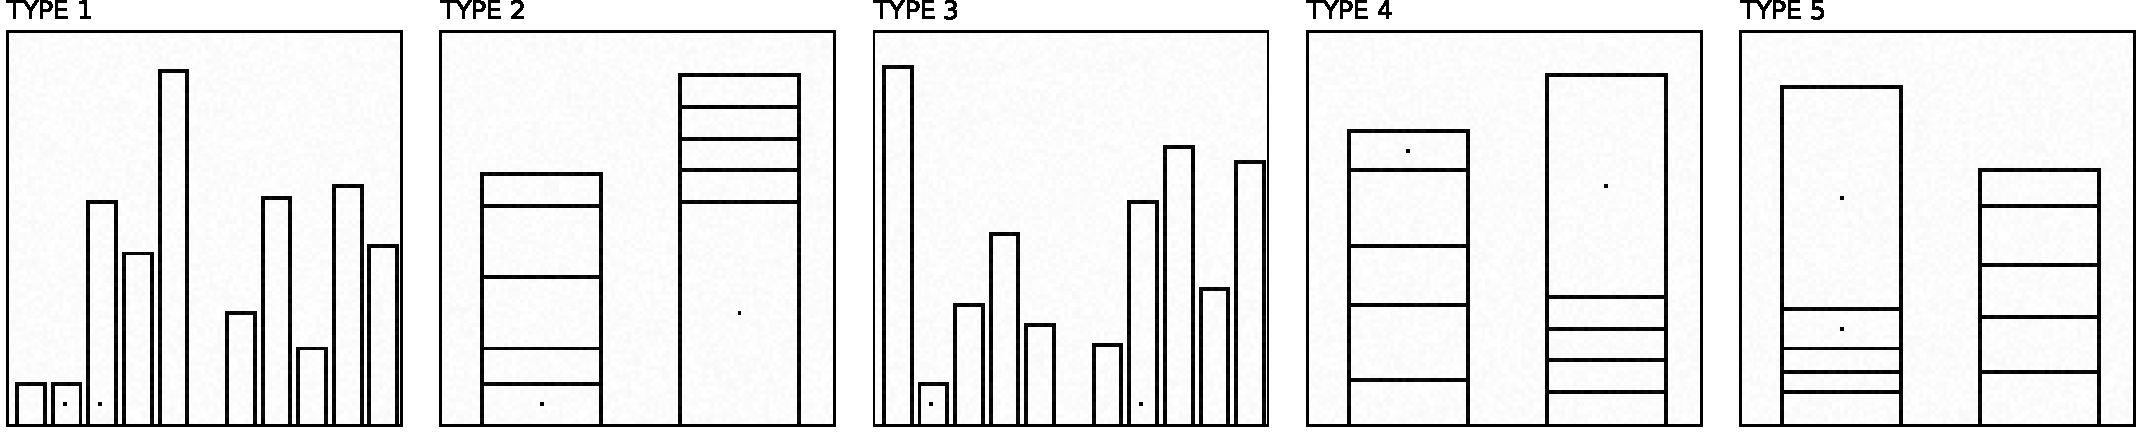
\includegraphics[width=\linewidth]{figure4_overview.pdf}
%   
%  \caption{\textbf{Position-Length Experiment.} (Not yet) Rasterized versions of the graphs of Cleveland and McGill's position-length experiment. The perceptual task involves comparing. the two dot-marked quantities across five different visual encodings of either grouped or divided bar charts. We evaluate which type of bar chart performs better with our neural networks as a combined classification and regression problem. The first task is to select which of the marked quantities is smaller (classification) and the second task is to specify how much smaller it is (regression).}
% \label{fig:position_length_experiment}
%\end{figure*}
%\begin{table}[h]
%\centering
%\caption{\textbf{Position-Length Experiment.} Rasterized versions of the graphs of Cleveland and McGill's position-length experiment. The perceptual task involves comparing the two dot-marked quantities across five different visual encodings of either grouped or divided bar charts. We evaluate which type of bar chart performs better with our neural networks. The two marked values are chosen from a set of ten pairs which defines the dual regression task. Since the other 8 values are chosen randomly, the parameter space for images of this experiment is massive.}
%\resizebox{\linewidth}{!}{
%\begin{tabular}{lllr}
% \toprule
% \multicolumn{2}{l}{~} & ~ & Permutations\\
% \midrule
% \raisebox{-.85\height}{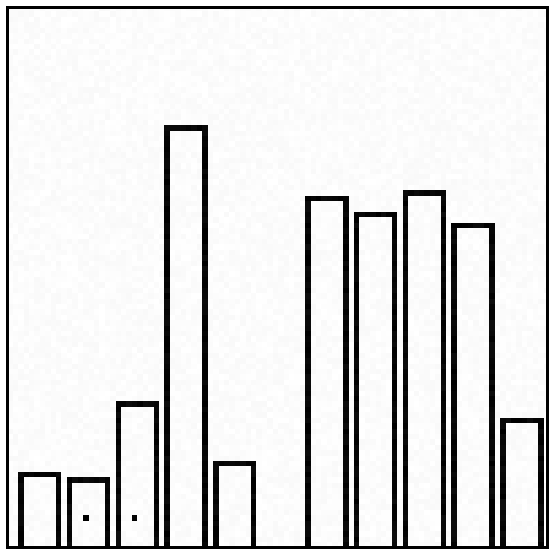
\includegraphics[width=.5in]{figure4_type_1.pdf}} & \makecell[tl]{Type 1: \emph{Grouped Bar Chart}\\~~~Perceptual Task: \emph{Position}\\~ \\~ \\} &~& \makecell[tr]{~\\ $9.20E+16$}\\
%
% \midrule
% \raisebox{-.85\height}{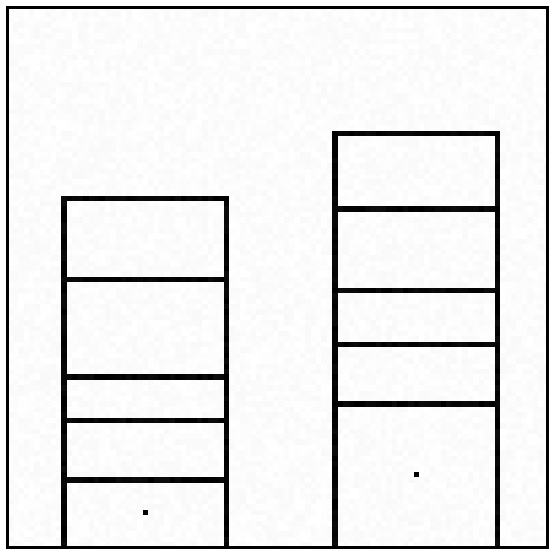
\includegraphics[width=.5in]{figure4_type_2.pdf}} & \makecell[tl]{Type 2: \emph{Divided Bar Chart}\\~~~Perceptual Task: \emph{Position}\\~ \\~ \\} &~& \makecell[tr]{~\\ $9.20E+16$}\\
% 
% \midrule
% \raisebox{-.85\height}{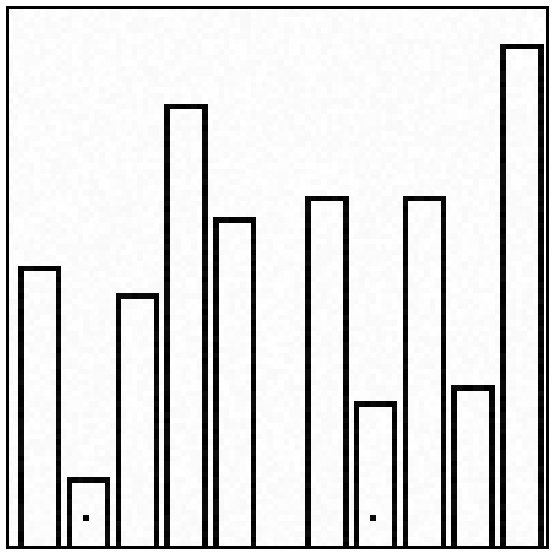
\includegraphics[width=.5in]{figure4_type_3.pdf}} & \makecell[tl]{Type 3: \emph{Grouped Bar Chart}\\~~~Perceptual Task: \emph{Position}\\~ \\~ \\} &~& \makecell[tr]{~\\ $9.20E+16$}\\
% 
% \midrule
% \raisebox{-.85\height}{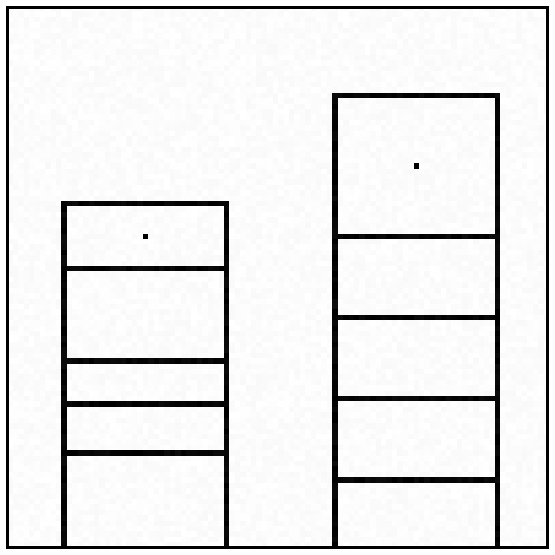
\includegraphics[width=.5in]{figure4_type_4.pdf}} & \makecell[tl]{Type 4: \emph{Divided Bar Chart}\\~~~Perceptual Task: \emph{Length}\\~ \\~ \\} &~& \makecell[tr]{~\\ $9.20E+16$}\\
% 
% \midrule
% \raisebox{-.85\height}{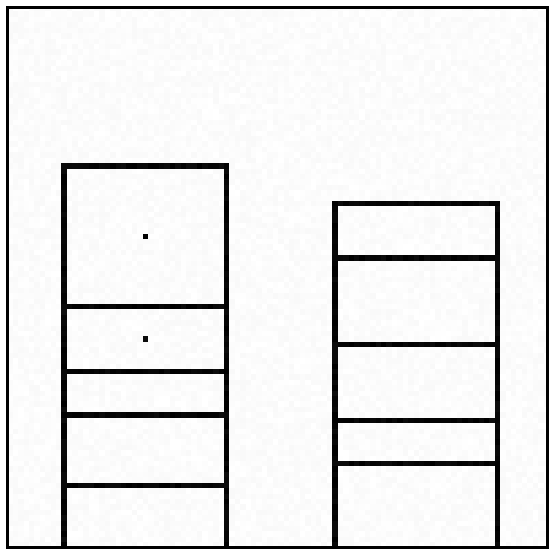
\includegraphics[width=.5in]{figure4_type_5.pdf}} & \makecell[tl]{Type 5: \emph{Divided Bar Chart}\\~~~Perceptual Task: \emph{Length}\\~ \\~ \\} &~& \makecell[tr]{~\\ $9.20E+16$}\\
%
% \bottomrule
%\end{tabular}
%}
%\label{tab:pos_length_parameters}
%\end{table}
%
%\subsection{Discussion}
%
%JT: Look at the relative difficulty of the tasks. In Cleveland and McGill, types 1-5 were post-ordered by their log error such that type 1 was easiest and type 5 was hardest. Is this still the case with our CNNs?

\vspace{-0.1cm}
\subsection{Results}

\begin{figure}[t]
  \centering
  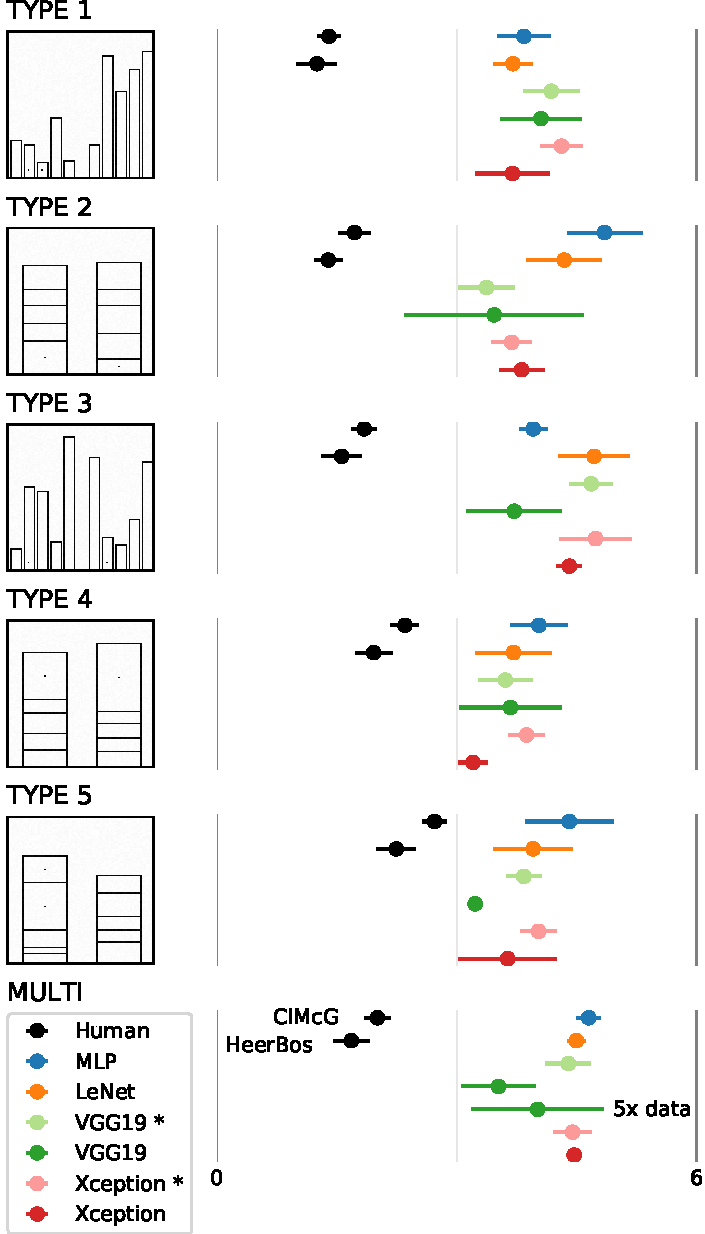
\includegraphics[width=0.90\linewidth]{figure4_mlae_with_multi_and_humans_all_NEW.pdf}
  \caption{\textbf{Computational results of the position-length experiment.} \textit{Left:} Type 1--5 stimuli for divided and grouped bar charts (as per Cleveland and McGill). \textit{Right:} MLAE and \change{bootstrapped} $95\%$ confidence intervals of our networks. Star * denotes networks using ImageNet weights. The last row shows `multi' networks trained on a random stream of types 1--5 \change{(plus VGG19 with $5\times$ training data)}. \change{We include human performance (black) from the original experiment (ClMcG, top) and from Heer and Bostock's crowdsourced studies (HeerBos, bottom).}}
  \label{fig:figure4_mlae}
\end{figure}

%\JT{State random performance.} 
%\JT{Mention Heer and Bostock's results in body text.}

\noindent\textbf{Perceptual Performance.} \change{Midmean random performance is at $MLAE=4.7$.} Average MLAE across our networks is: 
type 1 $MLAE= 3.956 $ ($SD= 0.274 $),
type 2 $MLAE= 3.952 $ ($SD= 0.441 $),
type 3 $MLAE= 4.349 $ ($SD= 0.367 $),
type 4 $MLAE= 3.668 $ ($SD= 0.256 $), and 
type 5 $MLAE= 3.902 $ ($SD= 0.253 $). This yields significance ($F_{4,25}=2.815, p<0.05$), but post-hoc comparisons show that only types 3 and 4 differ ($t_{10}=3.406, p<0.01$). Thus, our networks do not prefer a certain type on average, and so we \textbf{partially accept H3.1}. %Further, we do not replicate the same type difficulty ordering as Cleveland and McGill in their human studies.

Overall, our networks' performances are clearly worse than their human baselines. The problem space in these visual relation tasks is much larger than in the elementary perceptual tasks, resulting in average errors of $12$--$20\%$. Further, the finding from the elementary perceptual tasks that position and length judgments had approximately equivalent rank is consistent with these findings.
\\~\\
\noindent\textbf{Multi-task Network Performance.} In the original position-length experiment, humans were asked to judge visualizations across types 1-5. In the last row of Fig.~\ref{fig:figure4_mlae}, we average the human performances to create an average score across tasks. For our multi-task networks trained on all stimuli types, we record an average error across all classifiers of $MLAE=4.358$ ($SD=0.327$). Then, we compare against the average errors for all types, as reported above for perceptual performance. We reach significant differences ($F_{5,30}=3.454,p<0.05$). Post-hoc comparisons yield significant differences between the multi-task network and type 4 ($t_{10}=3.716, p<0.01$) and also to type 5 ($t_{10}=2.467, p<0.05$). Since the average MLAE is worse than all of types 1--5, and the distributions observe significant differences, we acknowledge that the multi-type task is harder for the networks than learning single types of encodings. We test whether there is insufficient training data for this task by providing five times more training data; however, this decreases performance. Thus, we \textbf{reject H3.2}. One promising exception is VGG trained from scratch, though performance has a wide variance across cross-validation sets.